\section{Ajánlási rendszer és Referenciák}

\newcounter{Acounter}
\newcommand{\sorSzamA}{\stepcounter{Acounter}\theAcounter}

\subsection{Referenciák}

A \textit{Segítség, építkezem!} weboldal lehetőséget ad a szakembereknek a referenciák felmutatására a korábbi munkáikról (\kovAzon{A\_\sorSzamA}), ezeket referenciáknak hívjuk. Ezek lehetnek:
\begin{enumerate}
  \item Szöveges dokumentum
  \item Kép
  \item Videó
  \item Használt alapanyagok és technológiák
\end{enumerate}

A referencia mindenképpen tartalmazza azokat az alapanyagokat és technológiákat, amelyeket a szakember meg tud határozni a projekttel kapcsolatban (\kovAzon{A\_\sorSzamA}).

Minden referenciát, amit a szakember a regisztráció során ad meg, egy adminisztrátor szerepkörrel rendelkező felhasználónak felül kell vizsglnia, hogy valódi-e. Szerződésekből visszakövethető, hogy valóban a szakember munkájáról van-e szó (\kovAzon{A\_\sorSzamA}). Minden olyan munka amit az oldalon rendeltek meg egy szakembertől, automatikusan megjelenik a szakembernél referenciaként. Ezt a referenciát később lehet ajánlásokkal bővíteni.

\subsection{Ajánlási rendszer}
Az ajánlási rendszer egy referencia szerzési lehetőség a szakembereknek. Az ügyfél adhat engedélyt a szakembernek, hogy az elkészült munkát más potenciális ügyfeleknek is személyesen megmutassa, vagy az elkészült munkáját valamilyen formában (pl. képek, videók) a javára fordíthassa. Az ajánlások több szintre bonthatóak (\kovAzon{A\_\sorSzamA}). Ezek a szintek korrelálnak a kedvezmények szintjeivel (\kovAzon{Ke\_1}). A szintek különböző mennyiségű és kategóriájú referenciákat követelnek meg. Az egymásra épülő szintek az alábbiak:
\begin{enumerate}
  \item Megemlítés, értékelés, egy-két fotó. Ezt minden referenciához szükséges megadni.
  \item Négy-öt fotó legalább, legyen köztük betéri fotó is (ha releváns)
  \item Videó.
  \item Kültéri, beltéri videós körbevezetés (ha releváns), pontos leírás.
  \item Személyes bemutatás.
\end{enumerate}
Ezeket az ajánlásokat a szakemberek felhasználhatják a referenciáikban. A szakember és az ügyfél az oldalon privát üzenetek segítségével megbeszélheti, az ajánlások részleteit (\kovAzon{A\_\sorSzamA}). Ajánlást akkor is írhat az ügyfél, ha a szakember nem társít hozzá kedvezményt (\kovAzon{A\_\sorSzamA}).

\begin{figure}[h]
	\centering
	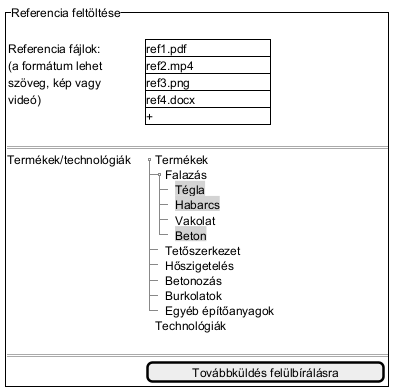
\includegraphics[scale=0.5]{img/referenciak.png}
	\caption{Referencia felvétele}
	\label{fig:ref}
\end{figure}